\documentclass[10pt,letterpaper]{article}

\renewcommand{\rmdefault}{\sfdefault}
\usepackage[parfill]{parskip}
\usepackage{fancyvrb}
\usepackage{fullpage}
\usepackage{graphicx}
\pagenumbering{gobble}


\begin{document}
\title{Enabling file auto-transfer on the Orbitrap Elite}
\author{Jeremy Volkening}
\date{\today}

\maketitle

The PC controller for the Orbitrap Elite has been set up such that RAW files
can be automatically transferred to a network share post-run and be available
to other computers in the Biotech network. To do so, certain options need to
be set during sequence submission. After selecting 'Run sequence...' in the
XCalibur software as usual, you will see the dialog as in Figure
\ref{screenshot}. The following command should be typed or pasted into the
text box marked ``A'' (note that you must use the full path to the program):

\begin{Verbatim}[frame=single]
C:\opt\cp_raw --raw %R
\end{Verbatim}

Additionally, the checkbox marked ``B'' should be checked. This will
automatically transfer the RAW file to the network share under the default
user directory ``other'' and a subdirectory named for the current date. Two
additional parameters are available but optional.  If ``\texttt{--mzml}'' is
given, the RAW file will additionally be converted to mzML and both files will
be copied to the network share. If ``\texttt{--user} \textit{USERNAME}'' is
given, the files will be copied into a directory named \textit{USERNAME}.
There is no enforcement on what user name is given, other than that it can
contain only letters, numbers, and undescore, so please don't mess with other
people's directories (however, as a safeguard, no existing files will be
overwritten by new ones).

As an additional example, the command

\begin{Verbatim}[frame=single]
C:\opt\cp_raw --raw %R --user foo --mzml
\end{Verbatim}

will copy both the RAW output and an mzML conversion to the network directory
under user ``foo'' and the current date.

\begin{figure}
  \centering
  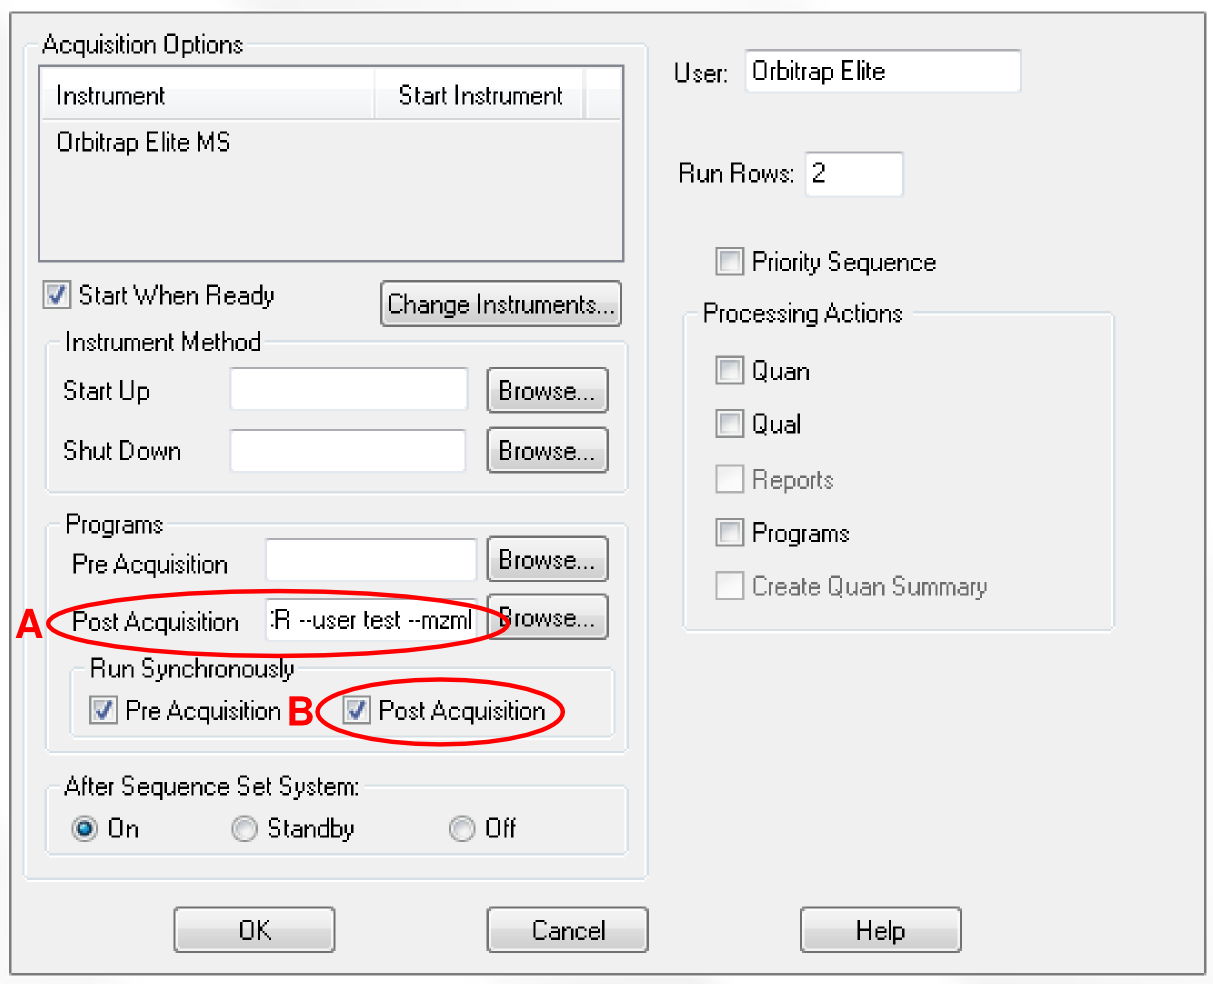
\includegraphics[width=0.4\textwidth]{screenshot}
  \caption{``Run Sequence..'' dialog highlighting relevant options}
  \label{screenshot}
\end{figure}

\end{document}
